% Generated from the entire threshold follow-up. Independent numerical audit is separate.
\textbf{Threshold-aware comparison.} All 54 engine and six reused-source conditions completed. Against Threshold Hot, the three engine-wide geometric-mean joint-cost ratios are 0.996, 1.000, 1.001. Against Threshold Hot Auto, the three engine-wide geometric-mean joint-cost ratios are 0.993, 1.000, 0.999. The registered broad engineering target is not supported. Table~\ref{tab:threshold-plans} includes all six plans; Fig.~\ref{fig:threshold-boundary} covers every engine cell. All ratios charge first use and the persistent receiver. Source-to-answer costs include aggregation and materialization on the unchanged encoded inputs.

\begin{table*}[t]
\centering
\caption{Six plans at $Q=100$. Engine columns give median [min, max] of three repeat-wise geometric-mean joint-cost ratios over all 18 cells. Dual/Auto denote the Threshold Hot controls. Uniform/Skew give median source-to-answer joint seconds. Decided counts combine true and false robust-threshold answers; they do not count beneficial policies.}
\label{tab:threshold-plans}\begingroup\fontsize{8}{9.4}\selectfont\setlength{\tabcolsep}{3pt}
\begin{tabular*}{\textwidth}{@{\extracolsep{\fill}}lrrrrr@{}}
\toprule
Plan & Engine / Dual & Engine / Auto & Uniform (s) & Skew (s) & Decided / 6,000\\
\midrule
Full Hot & 1.428 [1.418, 1.436] & 1.426 [1.418, 1.433] & 0.346 & 0.444 & 5,725\\
Threshold Hot & 1.000 [1.000, 1.000] & 0.999 [0.998, 1.000] & 0.495 & 0.312 & 5,749\\
Primal History & 0.992 [0.992, 0.992] & 0.991 [0.990, 0.992] & 0.497 & 0.315 & 5,751\\
Dual History & 1.006 [1.003, 1.010] & 1.005 [1.001, 1.010] & 0.511 & 0.313 & 5,749\\
Both Histories & 1.000 [0.996, 1.001] & 0.999 [0.993, 1.000] & 0.512 & 0.313 & 5,751\\
Threshold Hot Auto & 1.001 [1.000, 1.002] & 1.000 [1.000, 1.000] & 0.493 & 0.313 & 5,737\\
\bottomrule
\end{tabular*}
\endgroup

\end{table*}

\begin{figure*}[t]
\centering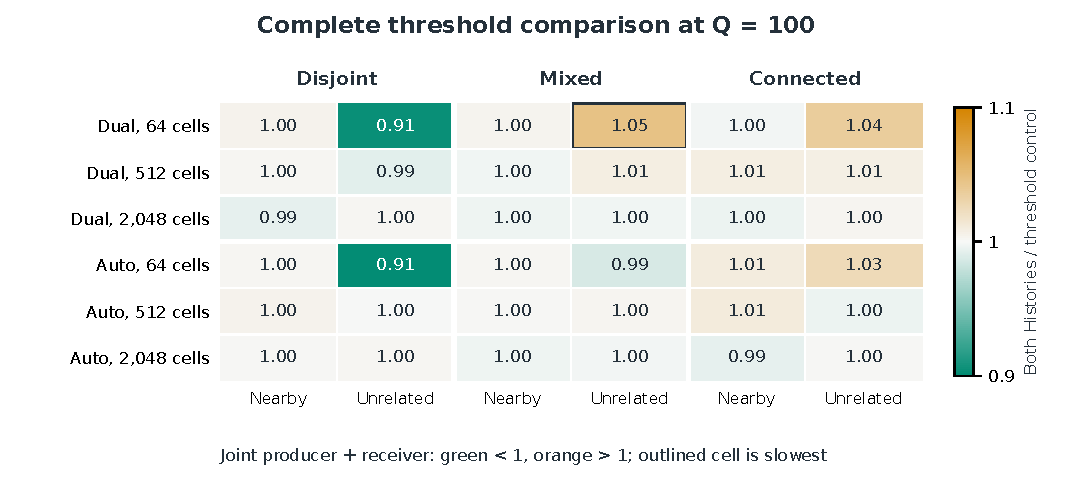
\includegraphics[width=\textwidth]{figures/threshold_boundary_v2.pdf}
\caption{Both Histories / Threshold Hot (Dual) or Threshold Hot Auto (Auto) in every engine cell. Entries are medians of three paired joint-cost ratios on one logarithmic color scale. The target applies to full-grid geometric means.}
\label{fig:threshold-boundary}
\end{figure*}

\textbf{What the histories contribute.} Both Histories returns 2,957 true, 2,794 false and 249 unknown answers. Earlier history serves 41/6,000 queries; the common last result serves 3,068/6,000. Initial-witness and box paths are recorded separately. Compared with Threshold Hot, it resolves 2 previously unknown answers but leaves 0 baseline-decided answers unknown. Compared with Threshold Hot Auto, it resolves 16 previously unknown answers but leaves 2 baseline-decided answers unknown. History changes answer availability slightly without the registered cost reduction. False means a checked counterexample within the view, as defined in Section~\ref{sec:threshold}. All 36,000 responses, including unknowns and 0 no-bound refusals, remain in the analysis.
